\documentclass[12pt]{article}
\usepackage{algo,fullpage,url,amssymb,epsfig,color,xspace,tikz,amsmath}
\usepackage{graphicx}
\usepackage[pdftitle={CS 240 Assignment 5},
pdfsubject={University of Waterloo, CS 240, Spring 2014},
pdfauthor={Romain Lebreton}]{hyperref}

%%%%%%%%%%%%%%%%%%%%% TIKZ %%%%%%%%%%%%%%%%%%%%%%%%%%%%%%
\usepackage{tkz-graph}
\usepackage{tikz}
\usepackage{tikz-qtree}
\makeatletter

\let\old@@children\@@children
\def\@@children{\futurelet\my@next\my@@children}
\def\my@@children{%
\ifx\my@next\missing\else
\expandafter\@gobble
\fi
\expandafter\old@@children}

\makeatother

\newcommand{\missing}{ \edge[draw=none]; {} }
\usetikzlibrary{chains}

% \snode{ID}{NUMBER} becomes \node{ID}[item]{\ensuremath{NUMBER}}
\newcommand{\snode}[2]{\node(#1)[item]{\ensuremath{#2}}}
\newcommand{\hlsnode}[2]{\node(#1)[item, fill = red!30]{\ensuremath{#2}}}

% \nodelabel{SUBSCRIPT} becomes \node[label]{\ensuremath{S_SUBSCRIPT}}
\newcommand{\nodelabel}[1]{\node[label]{\ensuremath{S_#1}}}
%%%%%%%%%%%%%%%%%%%%%%%%%%%%%%%%%%%%%%%%%%%%%%%%%%%%%%%%%

\renewcommand{\thesubsection}{Problem \arabic{subsection}}

\newcommand{\vs}{\textvisiblespace}

\begin{document}

\begin{center}
  {\Large\bf University of Waterloo}\\ \vspace{3mm}
  {\Large\bf CS240, Spring 2014}\\ \vspace{2mm}
  {\Large\bf Assignment 5 - Update 1}\\ \vspace{3mm}
  \textbf{Due Date: Wednesday, July 30, at 9:15am}
\end{center}

\definecolor{care}{rgb}{0,0,0}
\def\question#1{\item[\bf #1.]}
\def\part#1{\item[\bf #1)]}
\newcommand{\pc}[1]{\mbox{\textbf{#1}}} % pseudocode

%%%% NEW %%%
\textbf{Update 1: } We have added Problems 4 to 10 to cover 
range queries (module 7), text algorithms (module 8) and 
compression (module 9). 
All questions are written problems except problem 4.a) which is 
is a programming problem; submit your solution to 4.a) electronically
as a file named {\tt kdpartition.cpp}.
%%%%%%%%%%%%

Please read
\url{http://www.student.cs.uwaterloo.ca/~cs240/s14/guidelines.pdf} for
guidelines on submission.
Submit your solutions to written problems electronically as a PDF file with
name {\tt a05wp.pdf} using MarkUs. We will also accept individual
question files named {\tt a05q1w.pdf}, {\tt a05q2w.pdf}, $\dots$.

%%%%%%%%%%%%%%%%%%%%%%%%%%%%%%%%%%%%%%%%%%%%%%%%%%%%%%%%%%%%%%%%%%%%%%%%
\subsection{Hashing [3+3=6 marks]}
Consider a hash table dictionary with universe $U=\{0, 1, 2, \dots , 24\}$ and size $M =5$. If items with keys $k = 21, 3, 16, 1$ are inserted in that order, draw the resulting hash table if we resolve collisions using:

\begin{itemize}
\item Linear probing with $h(k) = (k+1)~mod~5$\\

- represents empty\\
\begin{tabular}{c|c|}
  \hline
  0 & 1\\
  \hline
  1 & -\\
  \hline
  2 & 21\\
  \hline
  3 & 16\\
  \hline
  4 & 3\\
  \hline
\end{tabular}

\item  Cuckoo hashing with $h_1(k) = k~mod~5$ and $h_2(k) =\lfloor k/5 \rfloor$

- represents empty\\
\begin{tabular}{c|c|}
  \hline
  0 & 3\\
  \hline
  1 & 1\\
  \hline
  2 & -\\
  \hline
  3 & 16\\
  \hline
  4 & 21\\
  \hline
\end{tabular}

\end{itemize}

%%%%%%%%%%%%%%%%%%%%%%%%%%%%%%%%%%%%%%%%%%%%%%%%%%%%%%%%%%%%%%%%%%%%%%%%
\subsection{Skip Lists [6+6+8=20 marks]}

\begin{figure}[!h]
  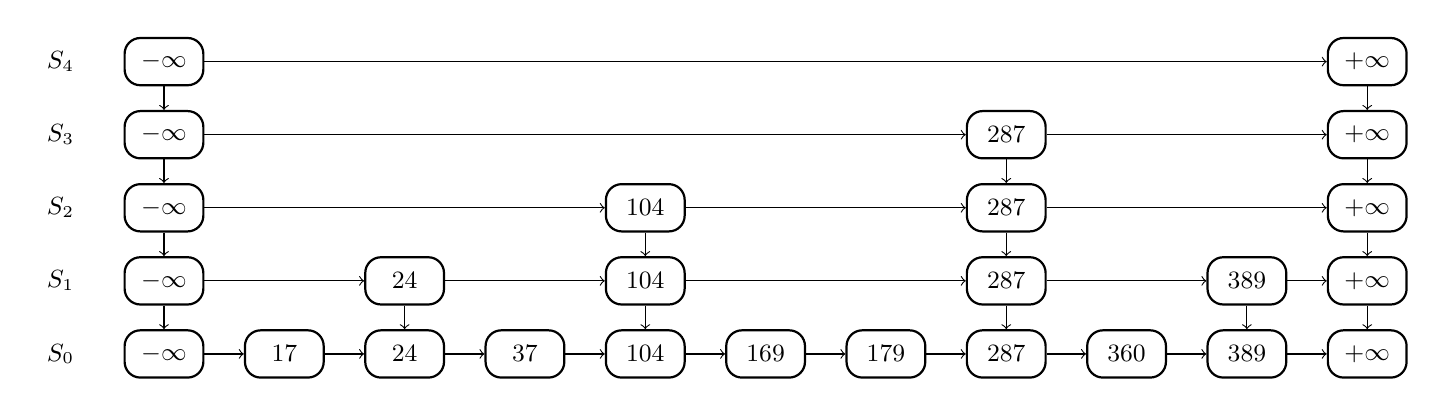
\begin{tikzpicture}[
      start chain,
      every node/.style={font=\small},
      item/.style={rectangle,minimum height=6mm,minimum width=10mm,
        rounded corners=2mm,thick,draw=black},
      label/.style={rectangle,minimum size=6mm},
      every join/.style={->}]
    % The nodes of the skip list are drawn in a matrix
    % \\ delimits the rows while & delimits the columns
    \matrix[row sep=3mm, column sep=5mm]{
      % Row 4: -infty ... +infty
      \nodelabel{4}; & \snode{4a}{-\infty}; & & & & & & & & & &\snode{4k}{+\infty};\\

      % Row 3: -infty ... 287 ... +infty
      \nodelabel{3}; & \snode{3a}{-\infty}; & & & & & & & \snode{3h}{287}; & & & \snode{3k}{+\infty};\\

      % Row 2: -infty ... 104 ... 287 ... +infty
      \nodelabel{2}; & \snode{2a}{-\infty}; & & & & \snode{2e}{104}; & & & \snode{2h}{287}; & & & \snode{2k}{+\infty};\\

      % Row 1: -infty - 24 - 104 - - 287 - 389 +infty
      \nodelabel{1}; & \snode{1a}{-\infty}; & & \snode{1c}{24}; & & \snode{1e}{104}; & & & \snode{1h}{287}; & & \snode{1j}{389}; & \snode{1k}{+\infty};\\

      % Row 0: -infty 17 24 37 104 169 179 287 360 389 +infty
      \nodelabel{0}; & \snode{0a}{-\infty}; & \snode{0b}{17}; & \snode{0c}{24}; & \snode{0d}{37}; & \snode{0e}{104}; & \snode{0f}{169}; & \snode{0g}{179}; & \snode{0h}{287}; & \snode{0i}{360}; & \snode{0j}{389}; & \snode{0k}{+\infty};\\
    };

    % Start chaining the nodes together
    {
      % Horizontal chains
      % Specify a starting node (by ID), and join to other nodes (by going "through" them in an unbroken line)
      % Eg row 2: Start at 2a, join 2e, join 2h, join 2i
      [start chain] \chainin(0a); \chainin(0b) [join]; \chainin(0c) [join]; \chainin(0d) [join]; \chainin(0e) [join]; \chainin(0f) [join]; \chainin(0g) [join]; \chainin(0h) [join]; \chainin(0i) [join]; \chainin(0j) [join]; \chainin(0k) [join];
      [start chain] \chainin(1a); \chainin(1c) [join]; \chainin(1e) [join]; \chainin(1h) [join]; \chainin(1j) [join]; \chainin(1k) [join];
      [start chain] \chainin(2a); \chainin(2e) [join]; \chainin(2h) [join]; \chainin(2k) [join];
      [start chain] \chainin(3a); \chainin(3h) [join]; \chainin(3k) [join];
      [start chain] \chainin(4a); \chainin(4k) [join];
    }
    {
      % Vertical chains
      % Need to be separate chains from the horizontal ones
      [start chain] \chainin(4a); \chainin(3a) [join]; \chainin(2a) [join]; \chainin(1a) [join]; \chainin(0a) [join];
      [start chain] \chainin(1c); \chainin(0c) [join];
      [start chain] \chainin(2e); \chainin(1e) [join]; \chainin(0e) [join];
      [start chain] \chainin(3h); \chainin(2h) [join]; \chainin(1h) [join]; \chainin(0h) [join];
      [start chain] \chainin(1j); \chainin(0j) [join];
      [start chain] \chainin(4k); \chainin(3k) [join]; \chainin(2k) [join]; \chainin(1k) [join]; \chainin(0k) [join];
    }
  \end{tikzpicture}
\end{figure}

\begin{enumerate}
\part{a} Consider the skip-list $S$ shown above. Show how $Search(S, 360)$ 
and  $Search(S, 17)$ proceeds. 
More specifically show at which order search visits the nodes of the skip list. 
Give only the successful search path, that is only the nodes that result into a 'go right' or 'go down'.
You should refer to the nodes using their keys and levels, e.g., 
you can say node 104 at level 1. The lowest level is $0$. 

\begin{enumerate}
\item Search(360):\\
$-\infty$ at level 4, go down\\
$-\infty$ at level 3, go right\\
$287$ at level 3, go down\\
287 at level 2, go down\\
287 at level 1, go down\\
287 at level 0, go right\\
360 at level 0\\

\item Search(17):\\
$-\infty$ at level 4, go down\\
$-\infty$ at level 3, go down\\
$-\infty$ at level 2, go down\\
$-\infty$ at level 1, go down\\
$-\infty$ at level 0, go right\\
17 at level 0
\end{enumerate}

\newpage

\part{b} Starting with an empty skip list, insert the seven keys
      $54, 15, 51,53, 47,68,36$.
      Draw your final answer as on the figure in 4(a).
      Use the following coin
      tosses to determine the  heights of towers (note, not every
      toss is necessarily used):
     $$T,T,H,H,T,H,T,H,H,T,H,H,T,T,H,T,H,H,T,T,H,H,H,T,\ldots$$

  \begin{figure}[h]
      % The nodes of the skip list are drawn in a matrix
    % \\ delimits the rows while & delimits the columns
  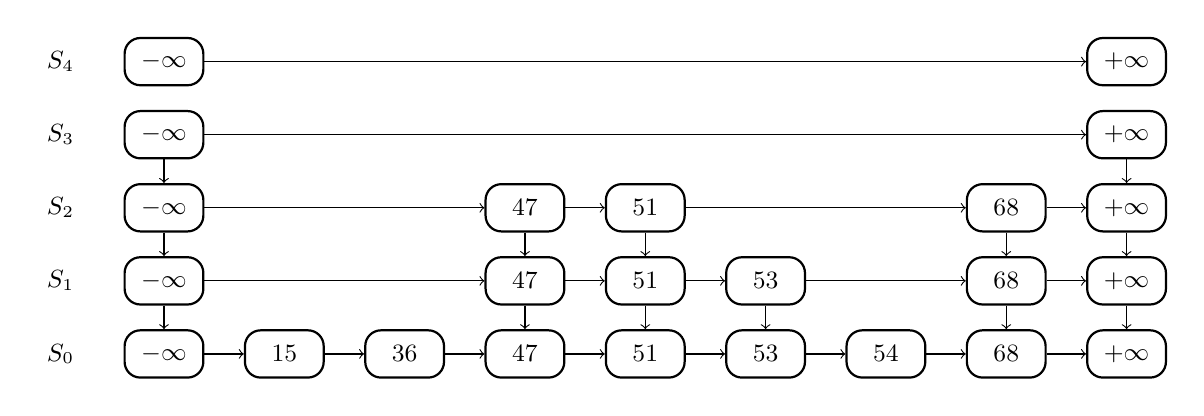
\begin{tikzpicture}[
      start chain,
      every node/.style={font=\small},
      item/.style={rectangle,minimum height=6mm,minimum width=10mm,
        rounded corners=2mm,thick,draw=black},
      label/.style={rectangle,minimum size=6mm},
      every join/.style={->}]
    % The nodes of the skip list are drawn in a matrix
    % \\ delimits the rows while & delimits the columns
    \matrix[row sep=3mm, column sep=5mm]{
      \nodelabel{4}; & \snode{4a}{-\infty}; & & & & & & & & \snode{4i}{+\infty};\\
      \nodelabel{3}; & \snode{3a}{-\infty}; & & & & & & & & \snode{3i}{+\infty};\\
      \nodelabel{2}; & \snode{2a}{-\infty}; & & & \snode{2d}{47}; & \snode{2e}{51}; & & & \snode{2h}{68}; & \snode{2i}{+\infty};\\
      \nodelabel{1}; & \snode{1a}{-\infty}; & & & \snode{1d}{47}; & \snode{1e}{51}; & \snode{1f}{53}; & & \snode{1h}{68}; & \snode{1i}{+\infty};\\
      \nodelabel{0}; & \snode{0a}{-\infty}; & \snode{0b}{15}; & \snode{0c}{36}; & \snode{0d}{47}; & \snode{0e}{51}; & \snode{0f}{53}; & \snode{0g}{54}; & \snode{0h}{68}; & \snode{0i}{+\infty};\\
    };

    {

      [start chain] \chainin(0a); \chainin(0b) [join]; \chainin(0c) [join]; \chainin(0d) [join]; \chainin(0e) [join]; \chainin(0f) [join]; \chainin(0g) [join]; \chainin(0h) [join]; \chainin(0i) [join];
      [start chain] \chainin(1a); \chainin(1d) [join]; \chainin(1e) [join]; \chainin(1f) [join]; \chainin(1h) [join]; \chainin(1i) [join];
      [start chain] \chainin(2a); \chainin(2d) [join]; \chainin(2e) [join]; \chainin(2h) [join]; \chainin(2i) [join];
      [start chain] \chainin(3a); \chainin(3i) [join];
      [start chain] \chainin(4a); \chainin(4i) [join];

    }
    {

      % Vertical chains
      % Need to be separate chains from the horizontal ones
      [start chain] \chainin(3a); \chainin(2a) [join]; \chainin(1a) [join]; \chainin(0a) [join];
      [start chain] \chainin(2d); \chainin(1d) [join]; \chainin(0d) [join];
      [start chain] \chainin(2e); \chainin(1e) [join]; \chainin(0e) [join];
      [start chain] \chainin(1f); \chainin(0f) [join];
      [start chain] \chainin(2h); \chainin(1h) [join]; \chainin(0h) [join];
      [start chain] \chainin(3i); \chainin(2i) [join]; \chainin(1i) [join]; \chainin(0i) [join];
    }
  \end{tikzpicture}
\end{figure}

\part{c} The worst case time for searching in a singly linked list
      is $\Theta(n)$.   Now consider a variation of  a skip list which
      has fixed height $h=3$ even though $n$ can become arbitrarily large.
      Level $S_0$ contains the keys $-\infty,k_1,k_2,\ldots,k_n,\infty$.
      Level $S_3$ contains only $-\infty$ and $\infty$.
      Describe subsets of keys that should be included in levels $S_1$
      and $S_2$ so that searching in the skip list has worst case cost
      $\Theta(n^{1/3})$.\\

      Put every multiple of $k_{n^{2/3}}$ from $k_0$ to $k_n$ on $S_2$, totalling $n^{1/3}$ + 1 of these multiples at this level. Put every multiple of $k_{n^{1/3}}$ from $k_0$ to $k_n$ on $S_1$, there would be $n^{2/3}$ + 1 of these multiples numbers at this level. No matter what number we search for, in the worst case the cost is $\Theta(n^{1/3})$.\\

      So if n was 64, put 0,16,32,48,64 on $S_2$ and 0,4,8,16..64 on $S_1$.\\\\

      In the worst case, we can only every perform $n^{1/3}$ - 1 shifts on $S_2$, then at max after moving down from $S_2$ we can perform $n^{1/3}$ - 1 shifts on $S_1$, and from $S_1$ you could then similarly at max perform $n^{1/3}$ - 1 shifts before finding the correct number or failing the search.

      This totals 3$n^{1/3}$ + c shifts, where c is a constant, which is $\Theta(n^{1/3})$ complexity.

\end{enumerate}

%%%%%%%%%%%%%%%%%%%%%%%%%%%%%%%%%%%%%%%%%%%%%%%%%%%%%%%%%%%%%%%%%%%%%%%%
\subsection{Quad Trees [5+5=10 marks]} 
For both parts of this question, use the convention that each
internal node of a quad tree has exactly four children, corresponding
to regions $NW$, $NE$, $SW$ and $SE$, in that order.

\begin{enumerate} 
\part{a} One of the applications of quad trees is for image
compression.  An image (picture) is recursively divided into quadrants
until the entire quadrant is only one color.  Using this rule,
draw the quad tree of the following image.  There are only three
colors (shades of gray).  For the leaves of the quad tree, use 1
to denote the lightest shade, 2 for the middle shade and 3 for the
darkest shade of gray.
\begin{center}
  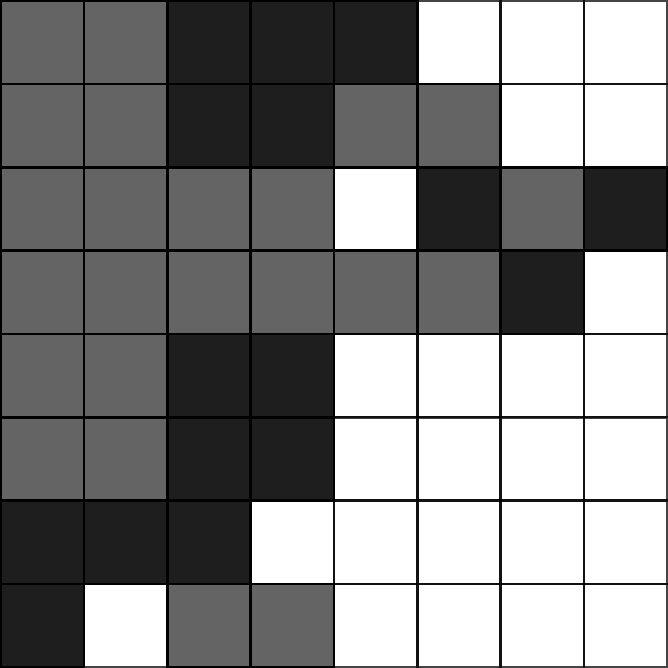
\includegraphics[width=3in]{QuadTreePic}
\end{center}

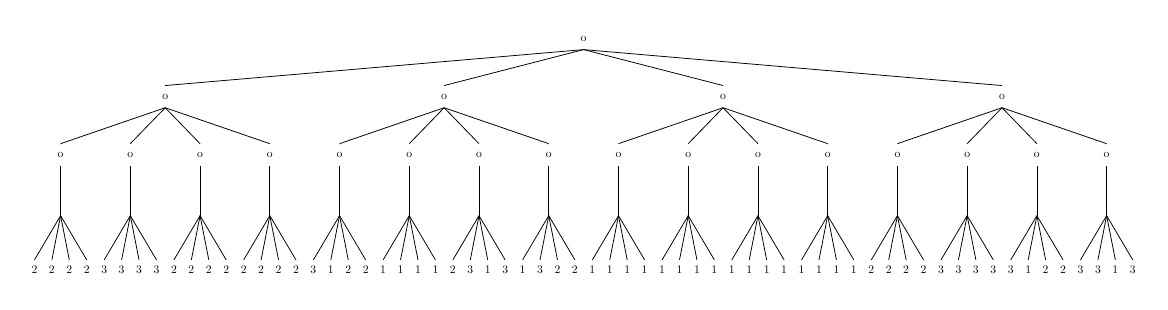
\begin{tikzpicture}[thick,scale=0.7, every node/.style={scale=0.6}]
\tikzset{execute at begin node=\strut}

\\If you can't see, zoom in:\\


\Tree [ .o 
        [ .o 
          [ .o 
            [ 2 2 2 2 ]
          ] 
          [ .o
            [ 3 3 3 3 ]
          ] 
          [ .o
            [ 2 2 2 2 ] 
          ] 
          [ .o 
            [ 2 2 2 2 ] 
          ] 
        ]
        [ .o 
          [ .o 
            [ 3 1 2 2 ]
          ] 
          [ .o
            [ 1 1 1 1 ]
          ] 
          [ .o
            [ 2 3 1 3 ] 
          ] 
          [ .o 
            [ 1 3 2 2 ] 
          ] 
        ]
        [ .o 
          [ .o 
            [ 1 1 1 1 ]
          ] 
          [ .o
            [ 1 1 1 1 ]
          ] 
          [ .o
            [ 1 1 1 1 ] 
          ] 
          [ .o 
            [ 1 1 1 1 ] 
          ] 
        ]
        [ .o 
          [ .o 
            [ 2 2 2 2 ]
          ] 
          [ .o
            [ 3 3 3 3 ]
          ] 
          [ .o
            [ 3 1 2 2 ] 
          ] 
          [ .o 
            [ 3 3 1 3 ] 
          ] 
        ]
      ] 
\end{tikzpicture}

\part{b} Give three 2-dimensional points such that the corresponding
quad tree has height exactly 9.  Give the (x,y) coordinates of the
three points and show the quad tree.  (Do not give the plane
partition.)

points: (1,1), (2,2), (1024,1024)

\begin{tikzpicture}[thick,scale=1.0, every node/.style={scale=0.6}]
\tikzset{execute at begin node=\strut}

\\If you can't see, zoom in:\\


\Tree [ .o 
        [
          {} (1024,1024) {}
          [ .o
            {} {} {}
            [ .o
              {} {} {}
              [ .o
                {} {} {}
                [ .o
                  {} {} {}
                  [ .o
                    {} {} {}
                    [ .o
                      {} {} {}
                      [ .o
                        {} {} {}
                        [ .o
                          {} {} {}
                          [ .o
                             {} (1,1) (2,2)
                          ]
                        ]
                      ]
                    ]
                  ]
                ]
              ]
            ]
          ]
        ]
      ]
\end{tikzpicture}



\end{enumerate}

%%%%%%%%%%%%%%%%%%%%%%%%%%%%%%%%%%%%%%%%%%%%%%%%%%%%%%%%%%%%%%%%%%%%%%%%
\subsection{$kd$-Tree Construction [15+5=20 marks]}
\begin{enumerate}
\part{a} Implement an $O(n\log n)$ algorithm to construct a $kd$-tree
for dimension 2.  Your algorithm should read $2n+1$ integers from
standard input, separated by white space or carriage return.  The first integer is the
number of points.  The remaining $2n$ integers are the $n$ points
themselves, according to their $x$ and $y$ coordinates.

Use the recipe on Slide 13 of Module 7 with the following modification on the split:
If the array $Px[0..n-1]$ for $n>1$ is storing points
sorted in increasing order according to their $x$-coordinate, then
the vertical splitting line goes through point $Px[mid]$, where
$mid = \lfloor n/2\rfloor$.  The root node contains $Px[mid]$, the
region to the left of the splitting
line include the points $Px[0..mid-1]$, and the region the the
right of the splitting line includes the points $Px[mid+1..n-1]$.

As explained in class, the idea of the algorithm is to first do some
preprocessing: sort the points on both their $x$ and $y$ coordinates.
For this preprocessing step you may use a standard library function;
assume that the sorting algorithm runs in time $O(n\log n)$. You may
also need some additional preprocessing.  Then call a recursive function
(which you create) to produce a tree like the one of Slide 14 of Module 7.
Actually, your program does not need to construct the tree, but rather
should just print to standard output the $n$ points stored in the nodes
of the tree in the order they are visited during an in-order traversal.
The coordinates of the point must be separated by a white space and we want 
one point per line.

Here is an example input:
\begin{verbatim}
3
3 4
2 2
1 1
\end{verbatim}
The points are $p_0,p_1,p_2 = (3,4),(2,2),(1,1)$. These three
points correspond to the following $kd$-tree:

\hfill 
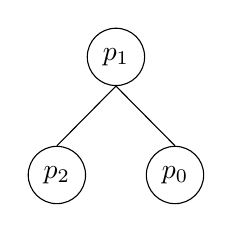
\begin{tikzpicture}[every node/.style={circle,draw}]
\node{$p_1$}
 child{ node{$p_2$}}
 child{ node{$p_0$}}
 ;
\end{tikzpicture}
\hfill \resizebox{30mm}{!}{\input{kdtreeExample.pdf_tex}}
\hfill \phantom{a}

Thus, for this example your algorithm should print out:
\begin{verbatim}
1 1
2 2
3 4 
\end{verbatim}
Your program {\bf must} run in time $O(n \log n)$.

To avoid all ambiguity in the construction of the k-d tree, you can assume that 
there will only be one point on each separating line. 
Therefore the choice of the median will always be unique, 
unlike the example of Slide 14 of Module 7 where $p_5$ and $p_6$ are on the same separating line. 
We will test your program only on such inputs.

\part{b} Justify the $O(n \log n)$ running time of your algorithm.  

One way to do this is to show that, after a preprocessing that involves sorting, 
you have a recursive algorithm whose running time on a sub-problem with $k$ points
satisfies the following recurrence: 
$$T(k) \leq T(\lfloor k/2\rfloor) + T(\lceil k/2 \rceil-1)+ O(k).$$
In other words, if you are splitting the region with a
vertical line according to $x$-coordinate, 
explain how you produce the two sets of points in each
region sorted according to their $y$-coordinate in time $O(k)$.
\end{enumerate}

%%%%%%%%%%%%%%%%%%%%%%%%%%%%%%%%%%%%%%%%%%%%%%%%%%%%%%%%%%%%%%%%%%%%%%%%
\subsection{Range tree [5+5+5=15 marks]}
\begin{enumerate}
\part{a} Draw the unique 2-dimensional range tree corresponding to points 
$[ 3, 4 ]$, $[ 10, 2 ]$, $[ 9, 9 ]$, $[ 5, 7 ]$, $[ 6, 1 ]$, $[ 0, 3 ]$, $[ 1, 8 ]$.
More specifically, we want you to draw all the trees $\tau$ and $\tau_{assoc}(p)$
for every point $p$.

\begin{figure}[ht!]
\centering
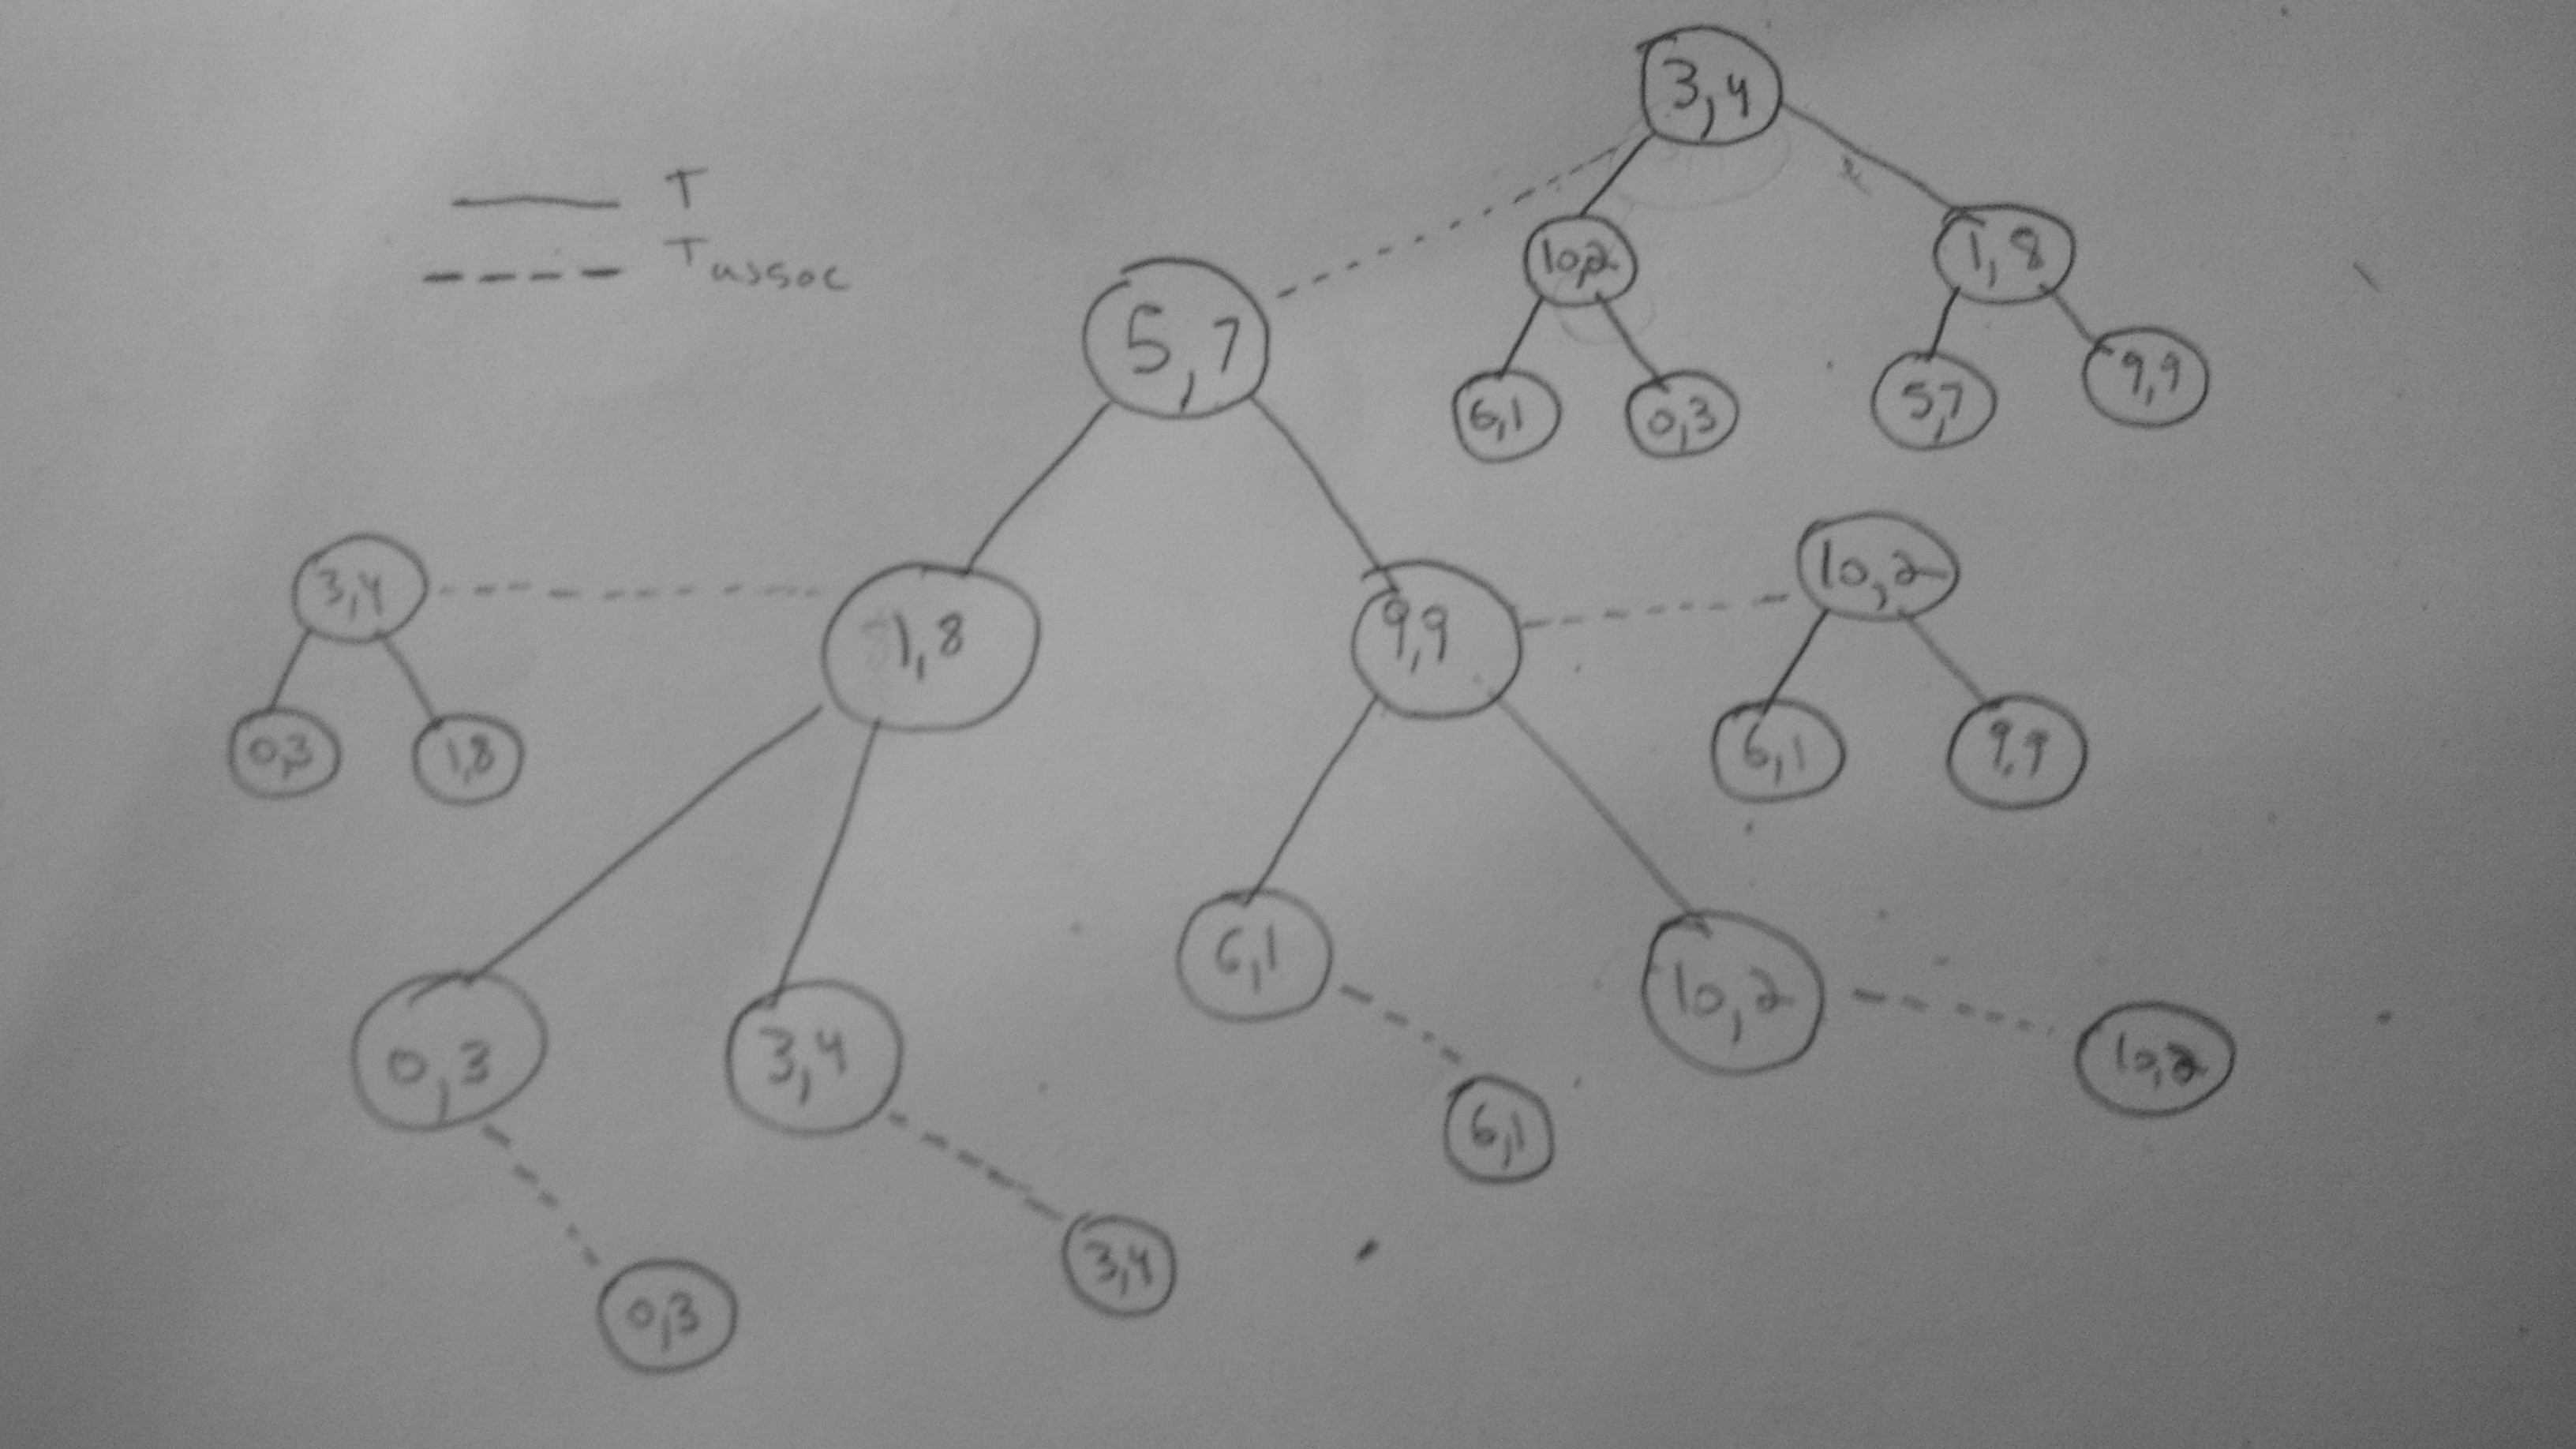
\includegraphics[width=170mm]{5a.jpg}
\label{overflow}
\end{figure}

\part{b} Assume that we have a set of $n$ numbers (not necessarily integers) and we are interested only in the number of points that lie in a range rather than in reporting all of them.  Describe how a 1-dimensional range tree (i.e., a balanced binary search tree) can be modified such that a range counting query can be performed in $O(\log{n})$ time
(independent of $k$). 

Modify the balanced binary tree T by introducing a counter on each node n that stores the number of nodes beneath the subtree of T with n as the root. When a new value is inserted into the tree, increase the counter on each of its ancestor nodes by one. This preprocessing of the tree allows a range counting query to be performed in $O(\log{n})$ time.\\\\

Now when a range query is performed, execute a BST-search on the left and right subtrees of the root in order to determine the boundary paths. Add 1 to the total of the range counting query for each boundary node along P1 and P2, which are the left and right paths traversed from the root by the query. For each boundary node visited, additionally increment the total by the counter stored on the top internal node of the boundary node. This way, rather than having to traverse the inside nodes reporting their values, the top inside node of each boundary node already knows the correct value to return, since every inside node should increment the total.\\\\

This modified procedure would then be a constant time operation to increment the count for each boundary node and then for its top internal node, which would run in the worst case the height of the tree for each path:

\begin{align*}
  &2\sum_{i=1}^{\log n} O(1)\\
  &=2(O(\log n))\\
  &=O(\log n)
\end{align*}

Therefore the modified range counting query can be performed in $O(\log{n})$ time.

\part{c} Now consider the 2-dimensional-case: We have a set of $n$ 2-dimensional points.  Given a query rectangle $R$, we want to find the number of points that lie in $R$.  Preprocess the $n$ points (by building an appropriate data structure) such that you can answer any of these counting queries in time $O((\log n)^2)$.

The solution to this problem uses a 2-dimensional range tree T of points (x,y) sorted by x-value, where T has an associated tree $\tau_{assoc}(p)$ sorted by y-value for every point p. Use the same preprocessing algorithm as in b) to store the number of nodes beneath p as a field on p. Perform a BST search based on the x-coordinates to determine the two boundary paths P1 and P2. Every time a boundary node m is visited, check the boundary node itself and if its y-coordinate also satisfies the range, increment the count by 1. Then perform a search just as in b) on the y-coordinates of each top inside node m's $\tau_{assoc}(m)$. The count returned by this operation is the number of inside nodes with a y-coordinate that falls within the range we are searching for, and since we already know that their x-coordinate is within the range, the returned count is added to the total.\\\\

This operation would be $O(\log n)$ time to create the boundary paths based on x-coordinate, then for each boundary node's top inside node, it could be at most another $O(\log n)$ complexity again to run the algorithm described in b) on a top inside node m's $\tau_{assoc}(m)$. Since there could be at most $\log n$ nodes in each boundary path P1 and P2 based on x-coordinate, we can describe the total cost as:

\begin{align*}
  &2\sum_{i=1}^{\log n} O(\log n)\\
  &=2O((\log n)^2)\\
  &=O((\log n)^2)
\end{align*}

Therefore in 2-dimensions, the modified range counting query can be performed in $O(\log{n})^2$ time.
\end{enumerate}

%%%%%%%%%%%%%%%%%%%%%%%%%%%%%%%%%%%%%%%%%%%%%%%%%%%%%%%%%%%%%%%%%%%%%%%%
\subsection{Tries [3+3+3+3+3=15 marks]}
\begin{itemize}
\part{a} Construct a trie on the following eight strings (include edge labels for clarity):\\ 000000, 1111111, 1111100, 011, 11011, 001111, 001100, 000100.

\begin{tikzpicture}[thick,scale=1.0, every node/.style={scale=0.6}]
\tikzset{execute at begin node=\strut}

\\If you can't see, zoom in:\\

\Tree [ .o ]
\end{tikzpicture}

\part{b} Draw the compressed trie equivalent to the trie in the previous part.
\part{c} Draw the compressed trie of the previous part after inserting 00011.
\part{d} Draw the compressed trie of part (b) after inserting 111011.
\part{e} Draw the compressed trie of part (b) after deleting 001100.
\end{itemize}

%%%%%%%%%%%%%%%%%%%%%%%%%%%%%%%%%%%%%%%%%%%%%%%%%%%%%%%%%%%%%
\subsection{KMP [6+6=12 marks]}
\begin{itemize}
\part{a} For each of the following pattern strings, determine the Knuth-Morris-Pratt
failure array:
\begin{enumerate}
\item $P = ${\tt~she sells seashells}
\item $P = ${\tt~abracadabracapabra}
\item $P = ${\tt~ababac}
\end{enumerate}
\part{b}
Show how to search for pattern $P=$\texttt{ababac} in the text $T=$\texttt{abcaabaabababacabcaa} using the KMP algorithm. Indicate in a table such as Table \ref{kmp} which characters of $P$ were compared with which characters of $T$. Follow the example on slide~25 in module~8. Place each character of $P$ in the column of the compared-to character of $T$.  Put brackets around the character if an actual comparison was not performed. You may not need all space in the table.
\end{itemize}

\begin{table}[!ht]
\Large{
\begin{center}
\begin{tabular}{|c|c|c|c|c|c|c|c|c|c|c|c|c|c|c|c|c|c|c|c|}
\hline
a&b&c&a&a&b&a&a&b&a&b&a&b&a&c&a&b&c&a&a\\
\hline
\hline
&&&&&&&&&&&&&&&&&&&\\
\hline
&&&&&&&&&&&&&&&&&&&\\
\hline
&&&&&&&&&&&&&&&&&&&\\
\hline
&&&&&&&&&&&&&&&&&&&\\
\hline
&&&&&&&&&&&&&&&&&&&\\
\hline
&&&&&&&&&&&&&&&&&&&\\
\hline
&&&&&&&&&&&&&&&&&&&\\
\hline
&&&&&&&&&&&&&&&&&&&\\
\hline
&&&&&&&&&&&&&&&&&&&\\
\hline
&&&&&&&&&&&&&&&&&&&\\
\hline
%\vdots&\vdots&\vdots&\vdots&\vdots&\vdots&\vdots&\vdots&\vdots&\vdots&\vdots&\vdots&\vdots&\vdots&\vdots&\vdots&\vdots&\vdots&\vdots&\vdots&\vdots\\
\end{tabular}
\end{center}}
\caption{Table for problem 3(b).}\label{kmp}
\end{table}

%%%%%%%%%%%%%%%%%%%%%%%%%%%%%%%%%%%%%%%%%%%%%%%%%%%%%%%%%%%%%
\subsection{Boyer-Moore [5+5+5=15 marks]}
\begin{itemize}
\part{a}
Compute the last-occurrence function $L$ for the pattern $P =$\texttt{~aabaab}.\\ Give your answer as a table as shown on slide 32 of module 8.
\part{b}
Compute the suffix skip array $S$ for the pattern $P =$\texttt{~aabaab}. \\Give your answer as a table as shown on slide 33 of module 8.
\part{c} Trace through the execution of Boyer-Moore algorithm for 
\begin{align*}
P &=& \tt{aabaab}\\
T &=& \tt{aaababdaabaaa}
\end{align*}
Indicate clearly the sequence of characters compared. Whenever a mismatch occurs, show clearly how the indices to $T$ and $P$ are computed.
\end{itemize}

%%%%%%%%%%%%%%%%%%%%%%%%%%%%%%%%%%%%%%%%%%%%%%%%%%%%%%%%%%%%%
\subsection{Suffix Trees [8 marks]} 
Draw the suffix tree corresponding to the text
$T =$\verb[ quisquam[.  Use the recipe of Slide~37 of Module~8.
Your suffix tree should look like the example on Slide~38.
Children of a node should be ordered alphabetically.

%%%%%%%%%%%%%%%%%%%%%%%%%%%%%%%%%%%%%%%%%%%%%%%%%%%%%%%%%%%%%
\subsection{Lempel-Ziv compression [8+1+1+1=11 marks]} 
After writing his memoirs, Foghorn Leghorn has decided to compress them 
using Lempel-Ziv compression with six bit codes. 
The code table is initialized with the codes 
$(a,000000)$, $(b,000001)$, $\dots$, $(z,011001)$, $({\vs},011010)$, 
$(',011011)$, $(, ,011100)$.
\begin{enumerate}
\part{a}Give the sequence of substrings that will be used during the compression 
of the opening sentence ``that's a joke, that's a joke, son, that's a joke''.
If we consider the example of Slide 26 of Module 9, we want you to answer 
$$[Y,O,!,{\vs},YO,U,!{\vs},YOU,R,{\vs}Y,O,YO,!].$$

You can assume that the dictionary is big enough to store 
all the substrings that we will encounter.

\part{b} What is the size in bits of the classical encoding of the original string considering that we would code every character from $a$ to ',' on 5 bits if we were not using LZW  ? 

\part{c} What is the size in bits of the compressed string ?

\part{d} Given the amount of repetition in the sentence above, comment on the quality of compression of LZW on this instance.

\end{enumerate}
\end{document}
